\documentclass{beamer}

\usepackage[utf8]{inputenc}
\usepackage[T1]{fontenc}
\usepackage{amsmath}
\usepackage{amssymb}
\usepackage{amsthm}
\usepackage{xcolor} % Pour colorer des symboles dans les équations
\usepackage{bbm}

\usepackage{tikz}
\usepackage{cite}

% Math operators
\newcommand{\scal}[2]{\left\langle #1 , #2 \right\rangle}
\DeclareMathOperator{\IR}{\mathbb{R}}
\DeclareMathOperator*{\argmin}{argmin}
\DeclareMathOperator{\One}{\mathbbm{1}}
\DeclareMathOperator{\Ccal}{\mathcal{C}}
\DeclareMathOperator{\logsumexp}{logsumexp}
\DeclareMathOperator{\diag}{diag}
\DeclareMathOperator{\KL}{KL}
\newcommand{\norm}[1]{\left\lVert #1 \right\rVert}
\renewcommand{\epsilon}{\varepsilon}

\title[Overrelaxed Sinkhorn--Knopp]{Overrelaxed Sinkhorn--Knopp Algorithm for Regularized Optimal Transport}

%
\author[A. THIBAULT]{
	Alexis THIBAULT, 
	L\'ena\"ic CHIZAT,\\
	Charles DOSSAL,
	Nicolas PAPADAKIS
}
\institute[OTML'17]{Optimal Transport and Machine Learning workshop \\ NIPS 2017}
\date{December 9, 2017}

\usetheme{Warsaw}


\begin{document}

\titlepage

\begin{frame}
\tableofcontents
\end{frame}

\section[Overrelaxing SK]{Overrelaxing the Sinkhorn--Knopp algorithm}

\subsection[SK algorithm]{The Sinkhorn--Knopp algorithm}
\begin{frame}{Regularized optimal transport}
Entropic regularization of optimal transport~:
\[
\gamma^* = \argmin_{\gamma \in \IR^{n_1 n_2}_+ \cap \Ccal_1 \cap \Ccal_2}
	\scal{c}{\gamma} + \epsilon \KL(\gamma,\One)
\]
\pause
Constraint sets~:
\begin{align}
\Ccal_1 &= \left\{ \gamma \mid A_1 \gamma = \mu^1 \right\},
&
\Ccal_2 &= \left\{ \gamma \mid A_2 \gamma = \mu^2 \right\}.
\end{align}
\pause
Kullback--Leibler divergence~:
\begin{equation}\label{KL}
\KL(\gamma,\xi) = \sum_{i,j} \gamma_{i,j} \left( \log \left( \frac{\gamma_{i,j}}{\xi_{i,j}} \right) -1  \right) + \sum_{i,j} \xi_{i,j}
\end{equation}
\end{frame}


\begin{frame}{Sinkhorn--Knopp algorithm}
\begin{columns}
\begin{column}{0.6\textwidth}
	
Bregman/Kullback-Leibler projection~:
\[
P_{\Ccal}(\xi) := \argmin_{\gamma \in \Ccal} \KL(\gamma,\xi).
\]
\pause
\begin{align*}
\gamma^0 &= e^{-c/\epsilon},\\
\gamma^* &= P_{\Ccal_1 \cap \Ccal_2}(\gamma^0).
\end{align*}
\pause
Sinkhorn--Knopp algorithm (SK)~:
\[
\lim P_{\Ccal_2}\circ P_{\Ccal_1} \circ \ldots \circ P_{\Ccal_2} \circ P_{\Ccal_1} (\gamma^0) = \gamma^*
\]
\end{column}

\begin{column}{0.4\textwidth}
	\centering
	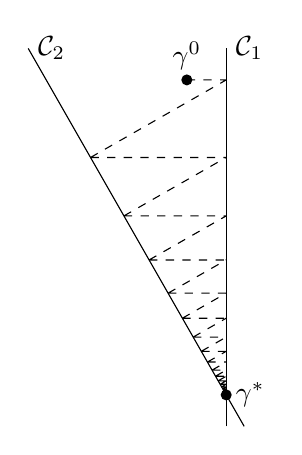
\begin{tikzpicture}
\fill (-0.500000,4.000000) circle (2pt) node[above] (gamma0) {$\gamma^0$};
\fill (0,0) circle (2pt) node[right] {$\gamma^*$};
\draw[dashed] (-0.500000,4.000000) -- (0.000000,4.000000)
(-1.723077,3.015385) -- (0.000000,4.000000)
(-1.723077,3.015385) -- (0.000000,3.015385)
(-1.298935,2.273136) -- (0.000000,3.015385)
(-1.298935,2.273136) -- (0.000000,2.273136)
(-0.979197,1.713595) -- (0.000000,2.273136)
(-0.979197,1.713595) -- (0.000000,1.713595)
(-0.738164,1.291787) -- (0.000000,1.713595)
(-0.738164,1.291787) -- (0.000000,1.291787)
(-0.556462,0.973809) -- (0.000000,1.291787)
(-0.556462,0.973809) -- (0.000000,0.973809)
(-0.419487,0.734102) -- (0.000000,0.973809)
(-0.419487,0.734102) -- (0.000000,0.734102)
(-0.316228,0.553400) -- (0.000000,0.734102)
(-0.316228,0.553400) -- (0.000000,0.553400)
(-0.238388,0.417178) -- (0.000000,0.553400)
(-0.238388,0.417178) -- (0.000000,0.417178)
(-0.179708,0.314488) -- (0.000000,0.417178)
(-0.179708,0.314488) -- (0.000000,0.314488)
(-0.135472,0.237076) -- (0.000000,0.314488)
(-0.135472,0.237076) -- (0.000000,0.237076)
(-0.102125,0.178719) -- (0.000000,0.237076)
(-0.102125,0.178719) -- (0.000000,0.178719)
(-0.076987,0.134726) -- (0.000000,0.178719)
(-0.076987,0.134726) -- (0.000000,0.134726)
(-0.058036,0.101563) -- (0.000000,0.134726)
(-0.058036,0.101563) -- (0.000000,0.101563)
(-0.043750,0.076563) -- (0.000000,0.101563)
(-0.043750,0.076563) -- (0.000000,0.076563)
(-0.032981,0.057717) -- (0.000000,0.076563)
(-0.032981,0.057717) -- (0.000000,0.057717)
(-0.024863,0.043509) -- (0.000000,0.057717)
(-0.024863,0.043509) -- (0.000000,0.043509)
(-0.018743,0.032799) -- (0.000000,0.043509)
(-0.018743,0.032799) -- (0.000000,0.032799)
(-0.014129,0.024726) -- (0.000000,0.032799)
(-0.014129,0.024726) -- (0.000000,0.024726)
(-0.010651,0.018639) -- (0.000000,0.024726)
(-0.010651,0.018639) -- (0.000000,0.018639)
(-0.008029,0.014051) -- (0.000000,0.018639)
(-0.008029,0.014051) -- (0.000000,0.014051)
(-0.006053,0.010592) -- (0.000000,0.014051)
(-0.006053,0.010592) -- (0.000000,0.010592)
(-0.004563,0.007985) -- (0.000000,0.010592)
(-0.004563,0.007985) -- (0.000000,0.007985)
(-0.003440,0.006020) -- (0.000000,0.007985)
(-0.003440,0.006020) -- (0.000000,0.006020)
(-0.002593,0.004538) -- (0.000000,0.006020)
(-0.002593,0.004538) -- (0.000000,0.004538)
(-0.001955,0.003421) -- (0.000000,0.004538)
(-0.001955,0.003421) -- (0.000000,0.003421)
(-0.001474,0.002579) -- (0.000000,0.003421)
(-0.001474,0.002579) -- (0.000000,0.002579)
(-0.001111,0.001944) -- (0.000000,0.002579)
(-0.001111,0.001944) -- (0.000000,0.001944)
(-0.000837,0.001465) -- (0.000000,0.001944)
(-0.000837,0.001465) -- (0.000000,0.001465)
(-0.000631,0.001105) -- (0.000000,0.001465)
(-0.000631,0.001105) -- (0.000000,0.001105)
(-0.000476,0.000833) -- (0.000000,0.001105)
(-0.000476,0.000833) -- (0.000000,0.000833)
(-0.000359,0.000628) -- (0.000000,0.000833)
(-0.000359,0.000628) -- (0.000000,0.000628)
(-0.000270,0.000473) -- (0.000000,0.000628)
(-0.000270,0.000473) -- (0.000000,0.000473)
(-0.000204,0.000357) -- (0.000000,0.000473)
(-0.000204,0.000357) -- (0.000000,0.000357)
(-0.000154,0.000269) -- (0.000000,0.000357)
(-0.000154,0.000269) -- (0.000000,0.000269)
(-0.000116,0.000203) -- (0.000000,0.000269)
(-0.000116,0.000203) -- (0.000000,0.000203)
(-0.000087,0.000153) -- (0.000000,0.000203)
(-0.000087,0.000153) -- (0.000000,0.000153)
(-0.000066,0.000115) -- (0.000000,0.000153)
(-0.000066,0.000115) -- (0.000000,0.000115)
(-0.000050,0.000087) -- (0.000000,0.000115)
(-0.000050,0.000087) -- (0.000000,0.000087)
(-0.000037,0.000065) -- (0.000000,0.000087)
(-0.000037,0.000065) -- (0.000000,0.000065)
(-0.000028,0.000049) -- (0.000000,0.000065)
(-0.000028,0.000049) -- (0.000000,0.000049)
(-0.000021,0.000037) -- (0.000000,0.000049)
(-0.000021,0.000037) -- (0.000000,0.000037)
(-0.000016,0.000028) -- (0.000000,0.000037)
(-0.000016,0.000028) -- (0.000000,0.000028)
(-0.000012,0.000021) -- (0.000000,0.000028)
(-0.000012,0.000021) -- (0.000000,0.000021)
(-0.000009,0.000016) -- (0.000000,0.000021)
(-0.000009,0.000016) -- (0.000000,0.000016)
(-0.000007,0.000012) -- (0.000000,0.000016)
(-0.000007,0.000012) -- (0.000000,0.000012)
(-0.000005,0.000009) -- (0.000000,0.000012)
(-0.000005,0.000009) -- (0.000000,0.000009)
(-0.000004,0.000007) -- (0.000000,0.000009)
(-0.000004,0.000007) -- (0.000000,0.000007)
(-0.000003,0.000005) -- (0.000000,0.000007)
(-0.000003,0.000005) -- (0.000000,0.000005)
(-0.000002,0.000004) -- (0.000000,0.000005)
(-0.000002,0.000004) -- (0.000000,0.000004)
(-0.000002,0.000003) -- (0.000000,0.000004)
(-0.000002,0.000003) -- (0.000000,0.000003)
(-0.000001,0.000002) -- (0.000000,0.000003)
(-0.000001,0.000002) -- (0.000000,0.000002)
(-0.000001,0.000002) -- (0.000000,0.000002)
(-0.000001,0.000002) -- (0.000000,0.000002)
(-0.000001,0.000001) -- (0.000000,0.000002)
(-0.000001,0.000001) -- (0.000000,0.000001)
(-0.000001,0.000001) -- (0.000000,0.000001)
(-0.000001,0.000001) -- (0.000000,0.000001)
(-0.000000,0.000001) -- (0.000000,0.000001)
(-0.000000,0.000001) -- (0.000000,0.000001)
(-0.000000,0.000001) -- (0.000000,0.000001)
(-0.000000,0.000001) -- (0.000000,0.000001)
(-0.000000,0.000000) -- (0.000000,0.000001)
(-0.000000,0.000000) -- (0.000000,0.000000)
(-0.000000,0.000000) -- (0.000000,0.000000)
(-0.000000,0.000000) -- (0.000000,0.000000)
(-0.000000,0.000000) -- (0.000000,0.000000)
(-0.000000,0.000000) -- (0.000000,0.000000)
(-0.000000,0.000000) -- (0.000000,0.000000)
(-0.000000,0.000000) -- (0.000000,0.000000)
(-0.000000,0.000000) -- (0.000000,0.000000)
(-0.000000,0.000000) -- (0.000000,0.000000)
(-0.000000,0.000000) -- (0.000000,0.000000)
(-0.000000,0.000000) -- (0.000000,0.000000)
(-0.000000,0.000000) -- (0.000000,0.000000)
(-0.000000,0.000000) -- (0.000000,0.000000)
(-0.000000,0.000000) -- (0.000000,0.000000)
(-0.000000,0.000000) -- (0.000000,0.000000)
(-0.000000,0.000000) -- (0.000000,0.000000)
(-0.000000,0.000000) -- (0.000000,0.000000)
(-0.000000,0.000000) -- (0.000000,0.000000)
(-0.000000,0.000000) -- (0.000000,0.000000)
(-0.000000,0.000000) -- (0.000000,0.000000)
(-0.000000,0.000000) -- (0.000000,0.000000)
(-0.000000,0.000000) -- (0.000000,0.000000)
(-0.000000,0.000000) -- (0.000000,0.000000)
(-0.000000,0.000000) -- (0.000000,0.000000)
(-0.000000,0.000000) -- (0.000000,0.000000)
(-0.000000,0.000000) -- (0.000000,0.000000)
(-0.000000,0.000000) -- (0.000000,0.000000)
(-0.000000,0.000000) -- (0.000000,0.000000)
(-0.000000,0.000000) -- (0.000000,0.000000)
(-0.000000,0.000000) -- (0.000000,0.000000)
(-0.000000,0.000000) -- (0.000000,0.000000)
(-0.000000,0.000000) -- (0.000000,0.000000)
(-0.000000,0.000000) -- (0.000000,0.000000)
(-0.000000,0.000000) -- (0.000000,0.000000)
(-0.000000,0.000000) -- (0.000000,0.000000)
(-0.000000,0.000000) -- (0.000000,0.000000)
(-0.000000,0.000000) -- (0.000000,0.000000)
(-0.000000,0.000000) -- (0.000000,0.000000)
(-0.000000,0.000000) -- (0.000000,0.000000)
(-0.000000,0.000000) -- (0.000000,0.000000)
(-0.000000,0.000000) -- (0.000000,0.000000)
(-0.000000,0.000000) -- (0.000000,0.000000)
(-0.000000,0.000000) -- (0.000000,0.000000)
(-0.000000,0.000000) -- (0.000000,0.000000)
(-0.000000,0.000000) -- (0.000000,0.000000)
(-0.000000,0.000000) -- (0.000000,0.000000)
(-0.000000,0.000000) -- (0.000000,0.000000)
(-0.000000,0.000000) -- (0.000000,0.000000)
(-0.000000,0.000000) -- (0.000000,0.000000)
(-0.000000,0.000000) -- (0.000000,0.000000)
(-0.000000,0.000000) -- (0.000000,0.000000)
(-0.000000,0.000000) -- (0.000000,0.000000)
(-0.000000,0.000000) -- (0.000000,0.000000)
(-0.000000,0.000000) -- (0.000000,0.000000)
(-0.000000,0.000000) -- (0.000000,0.000000)
(-0.000000,0.000000) -- (0.000000,0.000000)
(-0.000000,0.000000) -- (0.000000,0.000000)
(-0.000000,0.000000) -- (0.000000,0.000000)
(-0.000000,0.000000) -- (0.000000,0.000000)
(-0.000000,0.000000) -- (0.000000,0.000000)
(-0.000000,0.000000) -- (0.000000,0.000000)
(-0.000000,0.000000) -- (0.000000,0.000000)
(-0.000000,0.000000) -- (0.000000,0.000000)
(-0.000000,0.000000) -- (0.000000,0.000000)
(-0.000000,0.000000) -- (0.000000,0.000000)
(-0.000000,0.000000) -- (0.000000,0.000000)
(-0.000000,0.000000) -- (0.000000,0.000000)
(-0.000000,0.000000) -- (0.000000,0.000000)
(-0.000000,0.000000) -- (0.000000,0.000000)
(-0.000000,0.000000) -- (0.000000,0.000000)
(-0.000000,0.000000) -- (0.000000,0.000000)
(-0.000000,0.000000) -- (0.000000,0.000000)
(-0.000000,0.000000) -- (0.000000,0.000000)
(-0.000000,0.000000) -- (0.000000,0.000000)
(-0.000000,0.000000) -- (0.000000,0.000000)
(-0.000000,0.000000) -- (0.000000,0.000000)
(-0.000000,0.000000) -- (0.000000,0.000000)
(-0.000000,0.000000) -- (0.000000,0.000000)
(-0.000000,0.000000) -- (0.000000,0.000000)
(-0.000000,0.000000) -- (0.000000,0.000000)
(-0.000000,0.000000) -- (0.000000,0.000000)
(-0.000000,0.000000) -- (0.000000,0.000000)
(-0.000000,0.000000) -- (0.000000,0.000000)
(-0.000000,0.000000) -- (0.000000,0.000000)
(-0.000000,0.000000) -- (0.000000,0.000000)
(-0.000000,0.000000) -- (0.000000,0.000000)
;
\draw (-0.000000,-0.400000) -- (0.000000,4.400000) node[right] {$\mathcal{C}_1$};
\draw (0.228571,-0.400000) -- (-2.514286,4.400000) node[right] {$\mathcal{C}_2$};
\end{tikzpicture}

\end{column}
\end{columns}
\end{frame}

\begin{frame}{Limits of the SK algorithm}
Linear convergence rate $1-\eta$, $\eta > 0$.

\begin{columns}
	\begin{column}{0.5\textwidth}
		\centering
		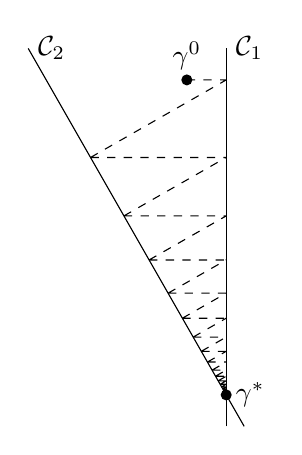
\begin{tikzpicture}
\fill (-0.500000,4.000000) circle (2pt) node[above] (gamma0) {$\gamma^0$};
\fill (0,0) circle (2pt) node[right] {$\gamma^*$};
\draw[dashed] (-0.500000,4.000000) -- (0.000000,4.000000)
(-1.723077,3.015385) -- (0.000000,4.000000)
(-1.723077,3.015385) -- (0.000000,3.015385)
(-1.298935,2.273136) -- (0.000000,3.015385)
(-1.298935,2.273136) -- (0.000000,2.273136)
(-0.979197,1.713595) -- (0.000000,2.273136)
(-0.979197,1.713595) -- (0.000000,1.713595)
(-0.738164,1.291787) -- (0.000000,1.713595)
(-0.738164,1.291787) -- (0.000000,1.291787)
(-0.556462,0.973809) -- (0.000000,1.291787)
(-0.556462,0.973809) -- (0.000000,0.973809)
(-0.419487,0.734102) -- (0.000000,0.973809)
(-0.419487,0.734102) -- (0.000000,0.734102)
(-0.316228,0.553400) -- (0.000000,0.734102)
(-0.316228,0.553400) -- (0.000000,0.553400)
(-0.238388,0.417178) -- (0.000000,0.553400)
(-0.238388,0.417178) -- (0.000000,0.417178)
(-0.179708,0.314488) -- (0.000000,0.417178)
(-0.179708,0.314488) -- (0.000000,0.314488)
(-0.135472,0.237076) -- (0.000000,0.314488)
(-0.135472,0.237076) -- (0.000000,0.237076)
(-0.102125,0.178719) -- (0.000000,0.237076)
(-0.102125,0.178719) -- (0.000000,0.178719)
(-0.076987,0.134726) -- (0.000000,0.178719)
(-0.076987,0.134726) -- (0.000000,0.134726)
(-0.058036,0.101563) -- (0.000000,0.134726)
(-0.058036,0.101563) -- (0.000000,0.101563)
(-0.043750,0.076563) -- (0.000000,0.101563)
(-0.043750,0.076563) -- (0.000000,0.076563)
(-0.032981,0.057717) -- (0.000000,0.076563)
(-0.032981,0.057717) -- (0.000000,0.057717)
(-0.024863,0.043509) -- (0.000000,0.057717)
(-0.024863,0.043509) -- (0.000000,0.043509)
(-0.018743,0.032799) -- (0.000000,0.043509)
(-0.018743,0.032799) -- (0.000000,0.032799)
(-0.014129,0.024726) -- (0.000000,0.032799)
(-0.014129,0.024726) -- (0.000000,0.024726)
(-0.010651,0.018639) -- (0.000000,0.024726)
(-0.010651,0.018639) -- (0.000000,0.018639)
(-0.008029,0.014051) -- (0.000000,0.018639)
(-0.008029,0.014051) -- (0.000000,0.014051)
(-0.006053,0.010592) -- (0.000000,0.014051)
(-0.006053,0.010592) -- (0.000000,0.010592)
(-0.004563,0.007985) -- (0.000000,0.010592)
(-0.004563,0.007985) -- (0.000000,0.007985)
(-0.003440,0.006020) -- (0.000000,0.007985)
(-0.003440,0.006020) -- (0.000000,0.006020)
(-0.002593,0.004538) -- (0.000000,0.006020)
(-0.002593,0.004538) -- (0.000000,0.004538)
(-0.001955,0.003421) -- (0.000000,0.004538)
(-0.001955,0.003421) -- (0.000000,0.003421)
(-0.001474,0.002579) -- (0.000000,0.003421)
(-0.001474,0.002579) -- (0.000000,0.002579)
(-0.001111,0.001944) -- (0.000000,0.002579)
(-0.001111,0.001944) -- (0.000000,0.001944)
(-0.000837,0.001465) -- (0.000000,0.001944)
(-0.000837,0.001465) -- (0.000000,0.001465)
(-0.000631,0.001105) -- (0.000000,0.001465)
(-0.000631,0.001105) -- (0.000000,0.001105)
(-0.000476,0.000833) -- (0.000000,0.001105)
(-0.000476,0.000833) -- (0.000000,0.000833)
(-0.000359,0.000628) -- (0.000000,0.000833)
(-0.000359,0.000628) -- (0.000000,0.000628)
(-0.000270,0.000473) -- (0.000000,0.000628)
(-0.000270,0.000473) -- (0.000000,0.000473)
(-0.000204,0.000357) -- (0.000000,0.000473)
(-0.000204,0.000357) -- (0.000000,0.000357)
(-0.000154,0.000269) -- (0.000000,0.000357)
(-0.000154,0.000269) -- (0.000000,0.000269)
(-0.000116,0.000203) -- (0.000000,0.000269)
(-0.000116,0.000203) -- (0.000000,0.000203)
(-0.000087,0.000153) -- (0.000000,0.000203)
(-0.000087,0.000153) -- (0.000000,0.000153)
(-0.000066,0.000115) -- (0.000000,0.000153)
(-0.000066,0.000115) -- (0.000000,0.000115)
(-0.000050,0.000087) -- (0.000000,0.000115)
(-0.000050,0.000087) -- (0.000000,0.000087)
(-0.000037,0.000065) -- (0.000000,0.000087)
(-0.000037,0.000065) -- (0.000000,0.000065)
(-0.000028,0.000049) -- (0.000000,0.000065)
(-0.000028,0.000049) -- (0.000000,0.000049)
(-0.000021,0.000037) -- (0.000000,0.000049)
(-0.000021,0.000037) -- (0.000000,0.000037)
(-0.000016,0.000028) -- (0.000000,0.000037)
(-0.000016,0.000028) -- (0.000000,0.000028)
(-0.000012,0.000021) -- (0.000000,0.000028)
(-0.000012,0.000021) -- (0.000000,0.000021)
(-0.000009,0.000016) -- (0.000000,0.000021)
(-0.000009,0.000016) -- (0.000000,0.000016)
(-0.000007,0.000012) -- (0.000000,0.000016)
(-0.000007,0.000012) -- (0.000000,0.000012)
(-0.000005,0.000009) -- (0.000000,0.000012)
(-0.000005,0.000009) -- (0.000000,0.000009)
(-0.000004,0.000007) -- (0.000000,0.000009)
(-0.000004,0.000007) -- (0.000000,0.000007)
(-0.000003,0.000005) -- (0.000000,0.000007)
(-0.000003,0.000005) -- (0.000000,0.000005)
(-0.000002,0.000004) -- (0.000000,0.000005)
(-0.000002,0.000004) -- (0.000000,0.000004)
(-0.000002,0.000003) -- (0.000000,0.000004)
(-0.000002,0.000003) -- (0.000000,0.000003)
(-0.000001,0.000002) -- (0.000000,0.000003)
(-0.000001,0.000002) -- (0.000000,0.000002)
(-0.000001,0.000002) -- (0.000000,0.000002)
(-0.000001,0.000002) -- (0.000000,0.000002)
(-0.000001,0.000001) -- (0.000000,0.000002)
(-0.000001,0.000001) -- (0.000000,0.000001)
(-0.000001,0.000001) -- (0.000000,0.000001)
(-0.000001,0.000001) -- (0.000000,0.000001)
(-0.000000,0.000001) -- (0.000000,0.000001)
(-0.000000,0.000001) -- (0.000000,0.000001)
(-0.000000,0.000001) -- (0.000000,0.000001)
(-0.000000,0.000001) -- (0.000000,0.000001)
(-0.000000,0.000000) -- (0.000000,0.000001)
(-0.000000,0.000000) -- (0.000000,0.000000)
(-0.000000,0.000000) -- (0.000000,0.000000)
(-0.000000,0.000000) -- (0.000000,0.000000)
(-0.000000,0.000000) -- (0.000000,0.000000)
(-0.000000,0.000000) -- (0.000000,0.000000)
(-0.000000,0.000000) -- (0.000000,0.000000)
(-0.000000,0.000000) -- (0.000000,0.000000)
(-0.000000,0.000000) -- (0.000000,0.000000)
(-0.000000,0.000000) -- (0.000000,0.000000)
(-0.000000,0.000000) -- (0.000000,0.000000)
(-0.000000,0.000000) -- (0.000000,0.000000)
(-0.000000,0.000000) -- (0.000000,0.000000)
(-0.000000,0.000000) -- (0.000000,0.000000)
(-0.000000,0.000000) -- (0.000000,0.000000)
(-0.000000,0.000000) -- (0.000000,0.000000)
(-0.000000,0.000000) -- (0.000000,0.000000)
(-0.000000,0.000000) -- (0.000000,0.000000)
(-0.000000,0.000000) -- (0.000000,0.000000)
(-0.000000,0.000000) -- (0.000000,0.000000)
(-0.000000,0.000000) -- (0.000000,0.000000)
(-0.000000,0.000000) -- (0.000000,0.000000)
(-0.000000,0.000000) -- (0.000000,0.000000)
(-0.000000,0.000000) -- (0.000000,0.000000)
(-0.000000,0.000000) -- (0.000000,0.000000)
(-0.000000,0.000000) -- (0.000000,0.000000)
(-0.000000,0.000000) -- (0.000000,0.000000)
(-0.000000,0.000000) -- (0.000000,0.000000)
(-0.000000,0.000000) -- (0.000000,0.000000)
(-0.000000,0.000000) -- (0.000000,0.000000)
(-0.000000,0.000000) -- (0.000000,0.000000)
(-0.000000,0.000000) -- (0.000000,0.000000)
(-0.000000,0.000000) -- (0.000000,0.000000)
(-0.000000,0.000000) -- (0.000000,0.000000)
(-0.000000,0.000000) -- (0.000000,0.000000)
(-0.000000,0.000000) -- (0.000000,0.000000)
(-0.000000,0.000000) -- (0.000000,0.000000)
(-0.000000,0.000000) -- (0.000000,0.000000)
(-0.000000,0.000000) -- (0.000000,0.000000)
(-0.000000,0.000000) -- (0.000000,0.000000)
(-0.000000,0.000000) -- (0.000000,0.000000)
(-0.000000,0.000000) -- (0.000000,0.000000)
(-0.000000,0.000000) -- (0.000000,0.000000)
(-0.000000,0.000000) -- (0.000000,0.000000)
(-0.000000,0.000000) -- (0.000000,0.000000)
(-0.000000,0.000000) -- (0.000000,0.000000)
(-0.000000,0.000000) -- (0.000000,0.000000)
(-0.000000,0.000000) -- (0.000000,0.000000)
(-0.000000,0.000000) -- (0.000000,0.000000)
(-0.000000,0.000000) -- (0.000000,0.000000)
(-0.000000,0.000000) -- (0.000000,0.000000)
(-0.000000,0.000000) -- (0.000000,0.000000)
(-0.000000,0.000000) -- (0.000000,0.000000)
(-0.000000,0.000000) -- (0.000000,0.000000)
(-0.000000,0.000000) -- (0.000000,0.000000)
(-0.000000,0.000000) -- (0.000000,0.000000)
(-0.000000,0.000000) -- (0.000000,0.000000)
(-0.000000,0.000000) -- (0.000000,0.000000)
(-0.000000,0.000000) -- (0.000000,0.000000)
(-0.000000,0.000000) -- (0.000000,0.000000)
(-0.000000,0.000000) -- (0.000000,0.000000)
(-0.000000,0.000000) -- (0.000000,0.000000)
(-0.000000,0.000000) -- (0.000000,0.000000)
(-0.000000,0.000000) -- (0.000000,0.000000)
(-0.000000,0.000000) -- (0.000000,0.000000)
(-0.000000,0.000000) -- (0.000000,0.000000)
(-0.000000,0.000000) -- (0.000000,0.000000)
(-0.000000,0.000000) -- (0.000000,0.000000)
(-0.000000,0.000000) -- (0.000000,0.000000)
(-0.000000,0.000000) -- (0.000000,0.000000)
(-0.000000,0.000000) -- (0.000000,0.000000)
(-0.000000,0.000000) -- (0.000000,0.000000)
(-0.000000,0.000000) -- (0.000000,0.000000)
(-0.000000,0.000000) -- (0.000000,0.000000)
(-0.000000,0.000000) -- (0.000000,0.000000)
(-0.000000,0.000000) -- (0.000000,0.000000)
(-0.000000,0.000000) -- (0.000000,0.000000)
(-0.000000,0.000000) -- (0.000000,0.000000)
(-0.000000,0.000000) -- (0.000000,0.000000)
(-0.000000,0.000000) -- (0.000000,0.000000)
(-0.000000,0.000000) -- (0.000000,0.000000)
(-0.000000,0.000000) -- (0.000000,0.000000)
(-0.000000,0.000000) -- (0.000000,0.000000)
(-0.000000,0.000000) -- (0.000000,0.000000)
(-0.000000,0.000000) -- (0.000000,0.000000)
(-0.000000,0.000000) -- (0.000000,0.000000)
(-0.000000,0.000000) -- (0.000000,0.000000)
;
\draw (-0.000000,-0.400000) -- (0.000000,4.400000) node[right] {$\mathcal{C}_1$};
\draw (0.228571,-0.400000) -- (-2.514286,4.400000) node[right] {$\mathcal{C}_2$};
\end{tikzpicture}
\\
		Large $\epsilon$
	\end{column}
	\begin{column}{0.5\textwidth}
		\centering
		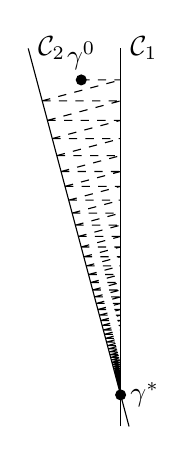
\begin{tikzpicture}
\fill (-0.500000,4.000000) circle (2pt) node[above] (gamma0) {$\gamma^0$};
\fill (0,0) circle (2pt) node[right] {$\gamma^*$};
\draw[dashed] (-0.500000,4.000000) -- (0.000000,4.000000)
(-0.995851,3.734440) -- (0.000000,4.000000)
(-0.995851,3.734440) -- (0.000000,3.734440)
(-0.929736,3.486510) -- (0.000000,3.734440)
(-0.929736,3.486510) -- (0.000000,3.486510)
(-0.868011,3.255041) -- (0.000000,3.486510)
(-0.868011,3.255041) -- (0.000000,3.255041)
(-0.810384,3.038938) -- (0.000000,3.255041)
(-0.810384,3.038938) -- (0.000000,3.038938)
(-0.756582,2.837183) -- (0.000000,3.038938)
(-0.756582,2.837183) -- (0.000000,2.837183)
(-0.706353,2.648822) -- (0.000000,2.837183)
(-0.706353,2.648822) -- (0.000000,2.648822)
(-0.659458,2.472967) -- (0.000000,2.648822)
(-0.659458,2.472967) -- (0.000000,2.472967)
(-0.615676,2.308787) -- (0.000000,2.472967)
(-0.615676,2.308787) -- (0.000000,2.308787)
(-0.574802,2.155506) -- (0.000000,2.308787)
(-0.574802,2.155506) -- (0.000000,2.155506)
(-0.536641,2.012402) -- (0.000000,2.155506)
(-0.536641,2.012402) -- (0.000000,2.012402)
(-0.501013,1.878799) -- (0.000000,2.012402)
(-0.501013,1.878799) -- (0.000000,1.878799)
(-0.467751,1.754065) -- (0.000000,1.878799)
(-0.467751,1.754065) -- (0.000000,1.754065)
(-0.436697,1.637613) -- (0.000000,1.754065)
(-0.436697,1.637613) -- (0.000000,1.637613)
(-0.407704,1.528891) -- (0.000000,1.637613)
(-0.407704,1.528891) -- (0.000000,1.528891)
(-0.380637,1.427388) -- (0.000000,1.528891)
(-0.380637,1.427388) -- (0.000000,1.427388)
(-0.355366,1.332624) -- (0.000000,1.427388)
(-0.355366,1.332624) -- (0.000000,1.332624)
(-0.331774,1.244151) -- (0.000000,1.332624)
(-0.331774,1.244151) -- (0.000000,1.244151)
(-0.309747,1.161552) -- (0.000000,1.244151)
(-0.309747,1.161552) -- (0.000000,1.161552)
(-0.289183,1.084436) -- (0.000000,1.161552)
(-0.289183,1.084436) -- (0.000000,1.084436)
(-0.269984,1.012440) -- (0.000000,1.084436)
(-0.269984,1.012440) -- (0.000000,1.012440)
(-0.252060,0.945225) -- (0.000000,1.012440)
(-0.252060,0.945225) -- (0.000000,0.945225)
(-0.235326,0.882471) -- (0.000000,0.945225)
(-0.235326,0.882471) -- (0.000000,0.882471)
(-0.219702,0.823884) -- (0.000000,0.882471)
(-0.219702,0.823884) -- (0.000000,0.823884)
(-0.205116,0.769186) -- (0.000000,0.823884)
(-0.205116,0.769186) -- (0.000000,0.769186)
(-0.191499,0.718120) -- (0.000000,0.769186)
(-0.191499,0.718120) -- (0.000000,0.718120)
(-0.178785,0.670444) -- (0.000000,0.718120)
(-0.178785,0.670444) -- (0.000000,0.670444)
(-0.166915,0.625933) -- (0.000000,0.670444)
(-0.166915,0.625933) -- (0.000000,0.625933)
(-0.155834,0.584377) -- (0.000000,0.625933)
(-0.155834,0.584377) -- (0.000000,0.584377)
(-0.145488,0.545580) -- (0.000000,0.584377)
(-0.145488,0.545580) -- (0.000000,0.545580)
(-0.135829,0.509359) -- (0.000000,0.545580)
(-0.135829,0.509359) -- (0.000000,0.509359)
(-0.126811,0.475543) -- (0.000000,0.509359)
(-0.126811,0.475543) -- (0.000000,0.475543)
(-0.118392,0.443972) -- (0.000000,0.475543)
(-0.118392,0.443972) -- (0.000000,0.443972)
(-0.110532,0.414496) -- (0.000000,0.443972)
(-0.110532,0.414496) -- (0.000000,0.414496)
(-0.103194,0.386978) -- (0.000000,0.414496)
(-0.103194,0.386978) -- (0.000000,0.386978)
(-0.096343,0.361286) -- (0.000000,0.386978)
(-0.096343,0.361286) -- (0.000000,0.361286)
(-0.089947,0.337301) -- (0.000000,0.361286)
(-0.089947,0.337301) -- (0.000000,0.337301)
(-0.083975,0.314907) -- (0.000000,0.337301)
(-0.083975,0.314907) -- (0.000000,0.314907)
(-0.078400,0.294000) -- (0.000000,0.314907)
(-0.078400,0.294000) -- (0.000000,0.294000)
(-0.073195,0.274482) -- (0.000000,0.294000)
(-0.073195,0.274482) -- (0.000000,0.274482)
(-0.068336,0.256259) -- (0.000000,0.274482)
(-0.068336,0.256259) -- (0.000000,0.256259)
(-0.063799,0.239246) -- (0.000000,0.256259)
(-0.063799,0.239246) -- (0.000000,0.239246)
(-0.059563,0.223362) -- (0.000000,0.239246)
(-0.059563,0.223362) -- (0.000000,0.223362)
(-0.055609,0.208533) -- (0.000000,0.223362)
(-0.055609,0.208533) -- (0.000000,0.208533)
(-0.051917,0.194689) -- (0.000000,0.208533)
(-0.051917,0.194689) -- (0.000000,0.194689)
(-0.048470,0.181763) -- (0.000000,0.194689)
(-0.048470,0.181763) -- (0.000000,0.181763)
(-0.045252,0.169696) -- (0.000000,0.181763)
(-0.045252,0.169696) -- (0.000000,0.169696)
(-0.042248,0.158430) -- (0.000000,0.169696)
(-0.042248,0.158430) -- (0.000000,0.158430)
(-0.039443,0.147912) -- (0.000000,0.158430)
(-0.039443,0.147912) -- (0.000000,0.147912)
(-0.036825,0.138092) -- (0.000000,0.147912)
(-0.036825,0.138092) -- (0.000000,0.138092)
(-0.034380,0.128924) -- (0.000000,0.138092)
(-0.034380,0.128924) -- (0.000000,0.128924)
(-0.032097,0.120365) -- (0.000000,0.128924)
(-0.032097,0.120365) -- (0.000000,0.120365)
(-0.029966,0.112374) -- (0.000000,0.120365)
(-0.029966,0.112374) -- (0.000000,0.112374)
(-0.027977,0.104913) -- (0.000000,0.112374)
(-0.027977,0.104913) -- (0.000000,0.104913)
(-0.026119,0.097948) -- (0.000000,0.104913)
(-0.026119,0.097948) -- (0.000000,0.097948)
(-0.024385,0.091445) -- (0.000000,0.097948)
(-0.024385,0.091445) -- (0.000000,0.091445)
(-0.022766,0.085374) -- (0.000000,0.091445)
(-0.022766,0.085374) -- (0.000000,0.085374)
(-0.021255,0.079706) -- (0.000000,0.085374)
(-0.021255,0.079706) -- (0.000000,0.079706)
(-0.019844,0.074415) -- (0.000000,0.079706)
(-0.019844,0.074415) -- (0.000000,0.074415)
(-0.018526,0.069474) -- (0.000000,0.074415)
(-0.018526,0.069474) -- (0.000000,0.069474)
(-0.017296,0.064862) -- (0.000000,0.069474)
(-0.017296,0.064862) -- (0.000000,0.064862)
(-0.016148,0.060556) -- (0.000000,0.064862)
(-0.016148,0.060556) -- (0.000000,0.060556)
(-0.015076,0.056535) -- (0.000000,0.060556)
(-0.015076,0.056535) -- (0.000000,0.056535)
(-0.014075,0.052782) -- (0.000000,0.056535)
(-0.014075,0.052782) -- (0.000000,0.052782)
(-0.013141,0.049278) -- (0.000000,0.052782)
(-0.013141,0.049278) -- (0.000000,0.049278)
(-0.012268,0.046006) -- (0.000000,0.049278)
(-0.012268,0.046006) -- (0.000000,0.046006)
(-0.011454,0.042952) -- (0.000000,0.046006)
(-0.011454,0.042952) -- (0.000000,0.042952)
(-0.010693,0.040100) -- (0.000000,0.042952)
(-0.010693,0.040100) -- (0.000000,0.040100)
(-0.009983,0.037438) -- (0.000000,0.040100)
(-0.009983,0.037438) -- (0.000000,0.037438)
(-0.009321,0.034952) -- (0.000000,0.037438)
(-0.009321,0.034952) -- (0.000000,0.034952)
(-0.008702,0.032632) -- (0.000000,0.034952)
(-0.008702,0.032632) -- (0.000000,0.032632)
(-0.008124,0.030466) -- (0.000000,0.032632)
(-0.008124,0.030466) -- (0.000000,0.030466)
(-0.007585,0.028443) -- (0.000000,0.030466)
(-0.007585,0.028443) -- (0.000000,0.028443)
(-0.007081,0.026555) -- (0.000000,0.028443)
(-0.007081,0.026555) -- (0.000000,0.026555)
(-0.006611,0.024792) -- (0.000000,0.026555)
(-0.006611,0.024792) -- (0.000000,0.024792)
(-0.006172,0.023146) -- (0.000000,0.024792)
(-0.006172,0.023146) -- (0.000000,0.023146)
(-0.005762,0.021609) -- (0.000000,0.023146)
(-0.005762,0.021609) -- (0.000000,0.021609)
(-0.005380,0.020174) -- (0.000000,0.021609)
(-0.005380,0.020174) -- (0.000000,0.020174)
(-0.005023,0.018835) -- (0.000000,0.020174)
(-0.005023,0.018835) -- (0.000000,0.018835)
(-0.004689,0.017585) -- (0.000000,0.018835)
(-0.004689,0.017585) -- (0.000000,0.017585)
(-0.004378,0.016417) -- (0.000000,0.017585)
(-0.004378,0.016417) -- (0.000000,0.016417)
(-0.004087,0.015327) -- (0.000000,0.016417)
(-0.004087,0.015327) -- (0.000000,0.015327)
(-0.003816,0.014310) -- (0.000000,0.015327)
(-0.003816,0.014310) -- (0.000000,0.014310)
(-0.003563,0.013360) -- (0.000000,0.014310)
(-0.003563,0.013360) -- (0.000000,0.013360)
(-0.003326,0.012473) -- (0.000000,0.013360)
(-0.003326,0.012473) -- (0.000000,0.012473)
(-0.003105,0.011645) -- (0.000000,0.012473)
(-0.003105,0.011645) -- (0.000000,0.011645)
(-0.002899,0.010872) -- (0.000000,0.011645)
(-0.002899,0.010872) -- (0.000000,0.010872)
(-0.002707,0.010150) -- (0.000000,0.010872)
(-0.002707,0.010150) -- (0.000000,0.010150)
(-0.002527,0.009476) -- (0.000000,0.010150)
(-0.002527,0.009476) -- (0.000000,0.009476)
(-0.002359,0.008847) -- (0.000000,0.009476)
(-0.002359,0.008847) -- (0.000000,0.008847)
(-0.002203,0.008259) -- (0.000000,0.008847)
(-0.002203,0.008259) -- (0.000000,0.008259)
(-0.002056,0.007711) -- (0.000000,0.008259)
(-0.002056,0.007711) -- (0.000000,0.007711)
(-0.001920,0.007199) -- (0.000000,0.007711)
(-0.001920,0.007199) -- (0.000000,0.007199)
(-0.001792,0.006721) -- (0.000000,0.007199)
(-0.001792,0.006721) -- (0.000000,0.006721)
(-0.001673,0.006275) -- (0.000000,0.006721)
(-0.001673,0.006275) -- (0.000000,0.006275)
(-0.001562,0.005858) -- (0.000000,0.006275)
(-0.001562,0.005858) -- (0.000000,0.005858)
(-0.001459,0.005469) -- (0.000000,0.005858)
(-0.001459,0.005469) -- (0.000000,0.005469)
(-0.001362,0.005106) -- (0.000000,0.005469)
(-0.001362,0.005106) -- (0.000000,0.005106)
(-0.001271,0.004767) -- (0.000000,0.005106)
(-0.001271,0.004767) -- (0.000000,0.004767)
(-0.001187,0.004451) -- (0.000000,0.004767)
(-0.001187,0.004451) -- (0.000000,0.004451)
(-0.001108,0.004155) -- (0.000000,0.004451)
;
\draw (-0.000000,-0.400000) -- (0.000000,4.400000) node[right] {$\mathcal{C}_1$};
\draw (0.106667,-0.400000) -- (-1.173333,4.400000) node[right] {$\mathcal{C}_2$};
\end{tikzpicture}
\\
		Small $\epsilon$
	\end{column}
\end{columns}

Small $\epsilon$ $\Longrightarrow$
very small $\eta$ $\Longrightarrow$
slow convergence
\end{frame}

\begin{frame}{Overrelaxation}
Bregman projection $\Longleftrightarrow$ scaling of rows/columns
\begin{align}\label{scaling}
P_{\Ccal_1}(\gamma) &= \diag(a) \gamma &\text{with}\quad
a &=  {\mu^1}\oslash{A_1 \gamma} \\
P_{\Ccal_2}(\gamma) &= \gamma \diag(b) &\text{with}\quad
b &= {\mu^2}\oslash{A_2 \gamma}\nonumber
\end{align}
\pause
Overrelaxed projections of parameter $\theta \in \IR$~:
\begin{align}\label{or_scaling}
P_{\Ccal_1}(\gamma) &= \diag(a)^\theta \gamma\\
P_{\Ccal_2}(\gamma) &= \gamma \diag(b)^\theta \nonumber
\end{align}
(element-wise exponentiation)
\end{frame}

\begin{frame}{Local study}
\begin{columns}
	\begin{column}{0.4\textwidth}
		\centering
		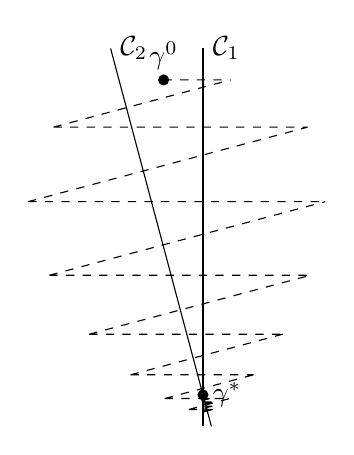
\begin{tikzpicture}
\fill (-0.500000,4.000000) circle (2pt) node[above] (gamma0) {$\gamma^0$};
\fill (0,0) circle (2pt) node[right] {$\gamma^*$};
\draw[dashed] (-0.500000,4.000000) -- (0.350000,4.000000)
(-1.898444,3.400415) -- (0.350000,4.000000)
(-1.898444,3.400415) -- (1.328911,3.400415)
(-2.219432,2.454190) -- (1.328911,3.400415)
(-2.219432,2.454190) -- (1.553603,2.454190)
(-1.950880,1.519661) -- (1.553603,2.454190)
(-1.950880,1.519661) -- (1.365616,1.519661)
(-1.444980,0.770169) -- (1.365616,1.519661)
(-1.444980,0.770169) -- (1.011486,0.770169)
(-0.919844,0.255148) -- (1.011486,0.770169)
(-0.919844,0.255148) -- (0.643891,0.255148)
(-0.486040,-0.046167) -- (0.643891,0.255148)
(-0.486040,-0.046167) -- (0.340228,-0.046167)
(-0.180221,-0.184954) -- (0.340228,-0.046167)
(-0.180221,-0.184954) -- (0.126154,-0.184954)
(0.004209,-0.217472) -- (0.126154,-0.184954)
(0.004209,-0.217472) -- (-0.002946,-0.217472)
(0.093772,-0.191681) -- (-0.002946,-0.217472)
(0.093772,-0.191681) -- (-0.065641,-0.191681)
(0.119666,-0.142266) -- (-0.065641,-0.191681)
(0.119666,-0.142266) -- (-0.083766,-0.142266)
(0.109394,-0.090756) -- (-0.083766,-0.142266)
(0.109394,-0.090756) -- (-0.076576,-0.090756)
(0.083372,-0.048103) -- (-0.076576,-0.090756)
(0.083372,-0.048103) -- (-0.058360,-0.048103)
(0.054625,-0.017974) -- (-0.058360,-0.048103)
(0.054625,-0.017974) -- (-0.038237,-0.017974)
(0.030058,0.000238) -- (-0.038237,-0.017974)
(0.030058,0.000238) -- (-0.021040,0.000238)
(0.012253,0.009116) -- (-0.021040,0.000238)
(0.012253,0.009116) -- (-0.008577,0.009116)
(0.001178,0.011717) -- (-0.008577,0.009116)
(0.001178,0.011717) -- (-0.000824,0.011717)
(-0.004475,0.010744) -- (-0.000824,0.011717)
(-0.004475,0.010744) -- (0.003133,0.010744)
(-0.006387,0.008205) -- (0.003133,0.010744)
(-0.006387,0.008205) -- (0.004471,0.008205)
(-0.006098,0.005387) -- (0.004471,0.008205)
(-0.006098,0.005387) -- (0.004268,0.005387)
(-0.004786,0.002973) -- (0.004268,0.005387)
(-0.004786,0.002973) -- (0.003350,0.002973)
(-0.003225,0.001219) -- (0.003350,0.002973)
(-0.003225,0.001219) -- (0.002258,0.001219)
(-0.001842,0.000126) -- (0.002258,0.001219)
(-0.001842,0.000126) -- (0.001289,0.000126)
(-0.000810,-0.000434) -- (0.001289,0.000126)
(-0.000810,-0.000434) -- (0.000567,-0.000434)
(-0.000149,-0.000625) -- (0.000567,-0.000434)
(-0.000149,-0.000625) -- (0.000105,-0.000625)
(0.000203,-0.000599) -- (0.000105,-0.000625)
(0.000203,-0.000599) -- (-0.000142,-0.000599)
(0.000337,-0.000471) -- (-0.000142,-0.000599)
(0.000337,-0.000471) -- (-0.000236,-0.000471)
(0.000338,-0.000318) -- (-0.000236,-0.000471)
(0.000338,-0.000318) -- (-0.000236,-0.000318)
(0.000273,-0.000182) -- (-0.000236,-0.000318)
(0.000273,-0.000182) -- (-0.000191,-0.000182)
(0.000189,-0.000080) -- (-0.000191,-0.000182)
(0.000189,-0.000080) -- (-0.000133,-0.000080)
(0.000112,-0.000015) -- (-0.000133,-0.000080)
(0.000112,-0.000015) -- (-0.000078,-0.000015)
(0.000052,0.000020) -- (-0.000078,-0.000015)
(0.000052,0.000020) -- (-0.000037,0.000020)
(0.000013,0.000033) -- (-0.000037,0.000020)
(0.000013,0.000033) -- (-0.000009,0.000033)
(-0.000008,0.000033) -- (-0.000009,0.000033)
(-0.000008,0.000033) -- (0.000006,0.000033)
(-0.000018,0.000027) -- (0.000006,0.000033)
(-0.000018,0.000027) -- (0.000012,0.000027)
(-0.000019,0.000019) -- (0.000012,0.000027)
(-0.000019,0.000019) -- (0.000013,0.000019)
(-0.000016,0.000011) -- (0.000013,0.000019)
(-0.000016,0.000011) -- (0.000011,0.000011)
(-0.000011,0.000005) -- (0.000011,0.000011)
(-0.000011,0.000005) -- (0.000008,0.000005)
(-0.000007,0.000001) -- (0.000008,0.000005)
(-0.000007,0.000001) -- (0.000005,0.000001)
(-0.000003,-0.000001) -- (0.000005,0.000001)
(-0.000003,-0.000001) -- (0.000002,-0.000001)
(-0.000001,-0.000002) -- (0.000002,-0.000001)
(-0.000001,-0.000002) -- (0.000001,-0.000002)
(0.000000,-0.000002) -- (0.000001,-0.000002)
(0.000000,-0.000002) -- (-0.000000,-0.000002)
(0.000001,-0.000002) -- (-0.000000,-0.000002)
(0.000001,-0.000002) -- (-0.000001,-0.000002)
(0.000001,-0.000001) -- (-0.000001,-0.000002)
(0.000001,-0.000001) -- (-0.000001,-0.000001)
(0.000001,-0.000001) -- (-0.000001,-0.000001)
(0.000001,-0.000001) -- (-0.000001,-0.000001)
(0.000001,-0.000000) -- (-0.000001,-0.000001)
(0.000001,-0.000000) -- (-0.000000,-0.000000)
(0.000000,-0.000000) -- (-0.000000,-0.000000)
(0.000000,-0.000000) -- (-0.000000,-0.000000)
(0.000000,0.000000) -- (-0.000000,-0.000000)
(0.000000,0.000000) -- (-0.000000,0.000000)
(0.000000,0.000000) -- (-0.000000,0.000000)
(0.000000,0.000000) -- (-0.000000,0.000000)
(-0.000000,0.000000) -- (-0.000000,0.000000)
(-0.000000,0.000000) -- (0.000000,0.000000)
(-0.000000,0.000000) -- (0.000000,0.000000)
(-0.000000,0.000000) -- (0.000000,0.000000)
(-0.000000,0.000000) -- (0.000000,0.000000)
(-0.000000,0.000000) -- (0.000000,0.000000)
(-0.000000,0.000000) -- (0.000000,0.000000)
(-0.000000,0.000000) -- (0.000000,0.000000)
(-0.000000,0.000000) -- (0.000000,0.000000)
(-0.000000,0.000000) -- (0.000000,0.000000)
(-0.000000,0.000000) -- (0.000000,0.000000)
(-0.000000,0.000000) -- (0.000000,0.000000)
(-0.000000,-0.000000) -- (0.000000,0.000000)
(-0.000000,-0.000000) -- (0.000000,-0.000000)
(-0.000000,-0.000000) -- (0.000000,-0.000000)
(-0.000000,-0.000000) -- (0.000000,-0.000000)
(-0.000000,-0.000000) -- (0.000000,-0.000000)
(-0.000000,-0.000000) -- (0.000000,-0.000000)
(0.000000,-0.000000) -- (0.000000,-0.000000)
(0.000000,-0.000000) -- (-0.000000,-0.000000)
(0.000000,-0.000000) -- (-0.000000,-0.000000)
(0.000000,-0.000000) -- (-0.000000,-0.000000)
(0.000000,-0.000000) -- (-0.000000,-0.000000)
(0.000000,-0.000000) -- (-0.000000,-0.000000)
(0.000000,-0.000000) -- (-0.000000,-0.000000)
(0.000000,-0.000000) -- (-0.000000,-0.000000)
(0.000000,-0.000000) -- (-0.000000,-0.000000)
(0.000000,-0.000000) -- (-0.000000,-0.000000)
(0.000000,-0.000000) -- (-0.000000,-0.000000)
(0.000000,-0.000000) -- (-0.000000,-0.000000)
(0.000000,0.000000) -- (-0.000000,-0.000000)
(0.000000,0.000000) -- (-0.000000,0.000000)
(0.000000,0.000000) -- (-0.000000,0.000000)
(0.000000,0.000000) -- (-0.000000,0.000000)
(-0.000000,0.000000) -- (-0.000000,0.000000)
(-0.000000,0.000000) -- (0.000000,0.000000)
(-0.000000,0.000000) -- (0.000000,0.000000)
(-0.000000,0.000000) -- (0.000000,0.000000)
(-0.000000,0.000000) -- (0.000000,0.000000)
(-0.000000,0.000000) -- (0.000000,0.000000)
(-0.000000,0.000000) -- (0.000000,0.000000)
(-0.000000,0.000000) -- (0.000000,0.000000)
(-0.000000,0.000000) -- (0.000000,0.000000)
(-0.000000,0.000000) -- (0.000000,0.000000)
(-0.000000,0.000000) -- (0.000000,0.000000)
(-0.000000,0.000000) -- (0.000000,0.000000)
(-0.000000,-0.000000) -- (0.000000,0.000000)
(-0.000000,-0.000000) -- (0.000000,-0.000000)
(-0.000000,-0.000000) -- (0.000000,-0.000000)
(-0.000000,-0.000000) -- (0.000000,-0.000000)
(0.000000,-0.000000) -- (0.000000,-0.000000)
(0.000000,-0.000000) -- (-0.000000,-0.000000)
(0.000000,-0.000000) -- (-0.000000,-0.000000)
(0.000000,-0.000000) -- (-0.000000,-0.000000)
(0.000000,-0.000000) -- (-0.000000,-0.000000)
(0.000000,-0.000000) -- (-0.000000,-0.000000)
(0.000000,-0.000000) -- (-0.000000,-0.000000)
(0.000000,-0.000000) -- (-0.000000,-0.000000)
(0.000000,-0.000000) -- (-0.000000,-0.000000)
(0.000000,-0.000000) -- (-0.000000,-0.000000)
(0.000000,-0.000000) -- (-0.000000,-0.000000)
(0.000000,-0.000000) -- (-0.000000,-0.000000)
(0.000000,0.000000) -- (-0.000000,-0.000000)
(0.000000,0.000000) -- (-0.000000,0.000000)
(0.000000,0.000000) -- (-0.000000,0.000000)
(0.000000,0.000000) -- (-0.000000,0.000000)
(-0.000000,0.000000) -- (-0.000000,0.000000)
(-0.000000,0.000000) -- (0.000000,0.000000)
(-0.000000,0.000000) -- (0.000000,0.000000)
(-0.000000,0.000000) -- (0.000000,0.000000)
(-0.000000,0.000000) -- (0.000000,0.000000)
(-0.000000,0.000000) -- (0.000000,0.000000)
(-0.000000,0.000000) -- (0.000000,0.000000)
(-0.000000,0.000000) -- (0.000000,0.000000)
(-0.000000,0.000000) -- (0.000000,0.000000)
(-0.000000,0.000000) -- (0.000000,0.000000)
(-0.000000,0.000000) -- (0.000000,0.000000)
(-0.000000,0.000000) -- (0.000000,0.000000)
(-0.000000,-0.000000) -- (0.000000,0.000000)
(-0.000000,-0.000000) -- (0.000000,-0.000000)
(-0.000000,-0.000000) -- (0.000000,-0.000000)
(-0.000000,-0.000000) -- (0.000000,-0.000000)
(0.000000,-0.000000) -- (0.000000,-0.000000)
(0.000000,-0.000000) -- (-0.000000,-0.000000)
(0.000000,-0.000000) -- (-0.000000,-0.000000)
(0.000000,-0.000000) -- (-0.000000,-0.000000)
(0.000000,-0.000000) -- (-0.000000,-0.000000)
(0.000000,-0.000000) -- (-0.000000,-0.000000)
(0.000000,-0.000000) -- (-0.000000,-0.000000)
(0.000000,-0.000000) -- (-0.000000,-0.000000)
(0.000000,-0.000000) -- (-0.000000,-0.000000)
(0.000000,-0.000000) -- (-0.000000,-0.000000)
(0.000000,-0.000000) -- (-0.000000,-0.000000)
(0.000000,-0.000000) -- (-0.000000,-0.000000)
(0.000000,0.000000) -- (-0.000000,-0.000000)
(0.000000,0.000000) -- (-0.000000,0.000000)
(0.000000,0.000000) -- (-0.000000,0.000000)
(0.000000,0.000000) -- (-0.000000,0.000000)
(0.000000,0.000000) -- (-0.000000,0.000000)
(0.000000,0.000000) -- (-0.000000,0.000000)
(-0.000000,0.000000) -- (-0.000000,0.000000)
(-0.000000,0.000000) -- (0.000000,0.000000)
(-0.000000,0.000000) -- (0.000000,0.000000)
;
\draw (-0.000000,-0.400000) -- (0.000000,4.400000) node[right] {$\mathcal{C}_1$};
\draw (0.106667,-0.400000) -- (-1.173333,4.400000) node[right] {$\mathcal{C}_2$};
\end{tikzpicture}
\\
		Typically take $\theta \in [1,2)$.
	\end{column}
	\begin{column}{0.6\textwidth}
		\pause
		Overrelaxation modifies each eigenvalue of $D_{\gamma^*}(P_{\Ccal_1} \circ P_{\Ccal_2})$.
		\begin{center}
			\includegraphics[width=6cm]{images/eigen_transform.png}
		\end{center}
		\pause
		Optimal parameter~: $\theta^* = \frac{2}{1+\sqrt{\eta}}$
	\end{column}
\end{columns}
\end{frame}


\end{document}
